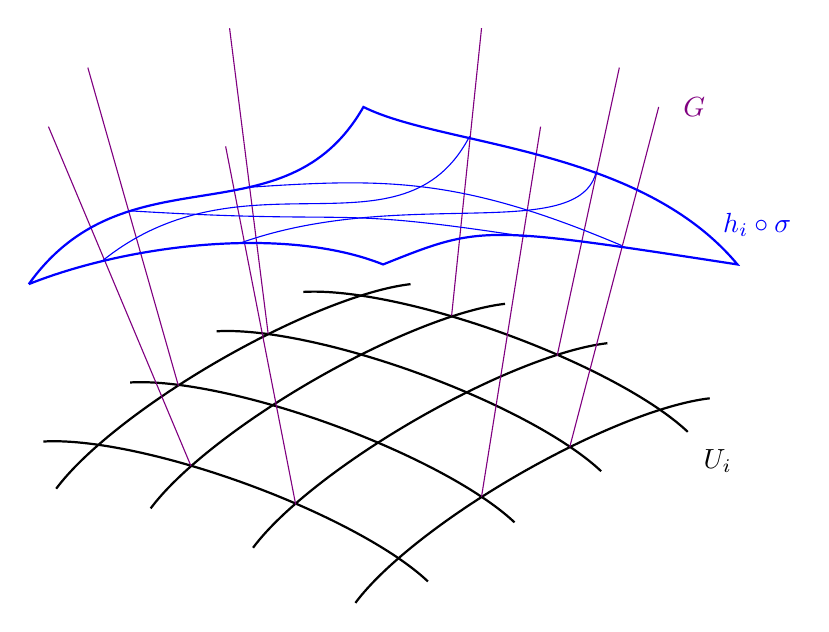
\begin{tikzpicture}%[scale=0.8]
	%\draw[opacity=0.1] (-4.5,-4.5) grid (4.5,4.5);

	%\draw (-1,-4)  .. controls (0,-2.5) and (1.5,-1.75) ..  (4,-2);

% BASE

	% gauche
	\draw[thick, xshift=1.3cm, yshift=-3.2cm, rotate=30]
		(3,0) arc [start angle=30, end angle =150, radius = 3, y radius = 0.75];
		
	\draw[thick, xshift=0cm, yshift=-2.5cm, rotate=30]
		(3,0) arc [start angle=30, end angle =150, radius = 3, y radius = 0.75];
		
	\draw[thick, xshift=-1.3cm, yshift=-2cm, rotate=30]
		(3,0) arc [start angle=30, end angle =150, radius = 3, y radius = 0.75];
		
	\draw[thick, xshift=-2.5cm, yshift=-1.75cm, rotate=30]
		(3,0) arc [start angle=30, end angle =150, radius = 3, y radius = 0.75];
		
	% droite
	\draw[thick, xshift=-2.5cm, yshift=-3cm, rotate=-20]
		(3,0) arc [start angle=30, end angle =150, radius = 3, y radius = 0.75];
	
	\draw[thick, xshift=-1.4cm, yshift=-2.25cm, rotate=-20]
		(3,0) arc [start angle=30, end angle =150, radius = 3, y radius = 0.75];
	
	\draw[thick, xshift=-0.3cm, yshift=-1.6cm, rotate=-20]
		(3,0) arc [start angle=30, end angle =150, radius = 3, y radius = 0.75];
	
	\draw[thick, xshift=0.8cm, yshift=-1.1cm, rotate=-20]
		(3,0) arc [start angle=30, end angle =150, radius = 3, y radius = 0.75];
	
	
% FIBRES

	\draw[violet] (-1.36,-3.05) -- (-2.25,1.5);
	\draw[violet] (1,-2.95) -- (1.75,1.75);
	
	\draw[violet] (-2.69,-2.56) -- (-4.5,1.75);
	\draw[violet] (2.12,-2.32) -- (3.25,2);
	
	\draw[violet] (-2.85,-1.54) -- (-4,2.5);
	\draw[violet] (1.96,-1.16) -- (2.75,2.5);
	
	\draw[violet] (-1.71,-0.88) -- (-2.2,3);
	\draw[violet] (0.62,-0.65) -- (1,3);
	
	
% SECTION

	%frame
	\draw[thick, blue] (-4.75,-0.25) .. controls (-3.5,1.5) and (-1.5,0.25) ..  
		(-0.5,2) .. controls (0.5,1.5) and (3,1.5) ..
		(4.25,0) .. controls (1,0.5) ..
		(-0.25,0) .. controls (-1.5,0.5) and (-3.5,0.25) ..
		(-4.75,-0.25);
		
	% coordo droite
	\draw[blue] (-3.45,0.68) .. controls (-0.5,0.5) and (-1,0.75) .. (1.58,0.35);
	\draw[blue] (-1.95,0.98) .. controls (-0.2,1.1) and (0.75,1.1) .. (2.78,0.24);
	
	%coordo gauche
	\draw[blue] (-3.81,0.05) .. controls (-2,1.5) and (0,0) .. (0.85,1.63);
	\draw[blue] (-2.04,0.28) .. controls (0,1) and (2.25,0.25) .. (2.46,1.19);
	
% NOTATION
	\draw (4,-2.5) node{ $U_i$};
	\draw (3.7,2) node{\color{violet} $G$};
	\draw (4.5,0.5) node{\color{blue} $h_i \circ \sigma$};
	
\end{tikzpicture}